\section{Watchdogs}

A watchdog timer is a critical component, either internal or external, designed to monitor the proper functioning of embedded systems.
It detects software anomalies and takes corrective actions, such as resetting or restarting the processor, to recover from system faults.
This functionality is essential for ensuring system reliability and is often referred to as Computer Operating Properly (COP).

In the context of the Internet of Things (IoT), where billions of devices are deployed in the field, manual intervention by a technician is often impractical. 
IoT systems must be self-reliant, capable of detecting and recovering from faults without human involvement. 
Watchdog timers play a pivotal role in this automated fault recovery.

Watchdog timers come in various forms, including simple timers, windowed timers, and more advanced smart watchdogs. 
They may be integrated as part of a microcontroller (either as hardware or software), exist as external hardware components, or even be standalone microcontrollers with their own hardware and software. 
Regardless of the type, the primary function of any watchdog timer is to continuously monitor system health and recover the system in case of failure. 
Each type of watchdog presents unique characteristics and design challenges that developers must consider to ensure a robust and fault-tolerant IoT system.

\subsection{Structure}
In normal operation, the system regularly "kicks" or resets the watchdog timer to prevent it from reaching its timeout. 
If a hardware fault or software error occurs, the system may fail to reset the timer. 
In such a case, the watchdog will time out and generate a corrective action, often in the form of a timeout signal.

However, the response to a timeout is not always a simple system reset. 
Corrective actions may vary depending on the fault and may include placing the system in a safe state before attempting to restore normal operation.
\begin{figure}[H]
    \centering
    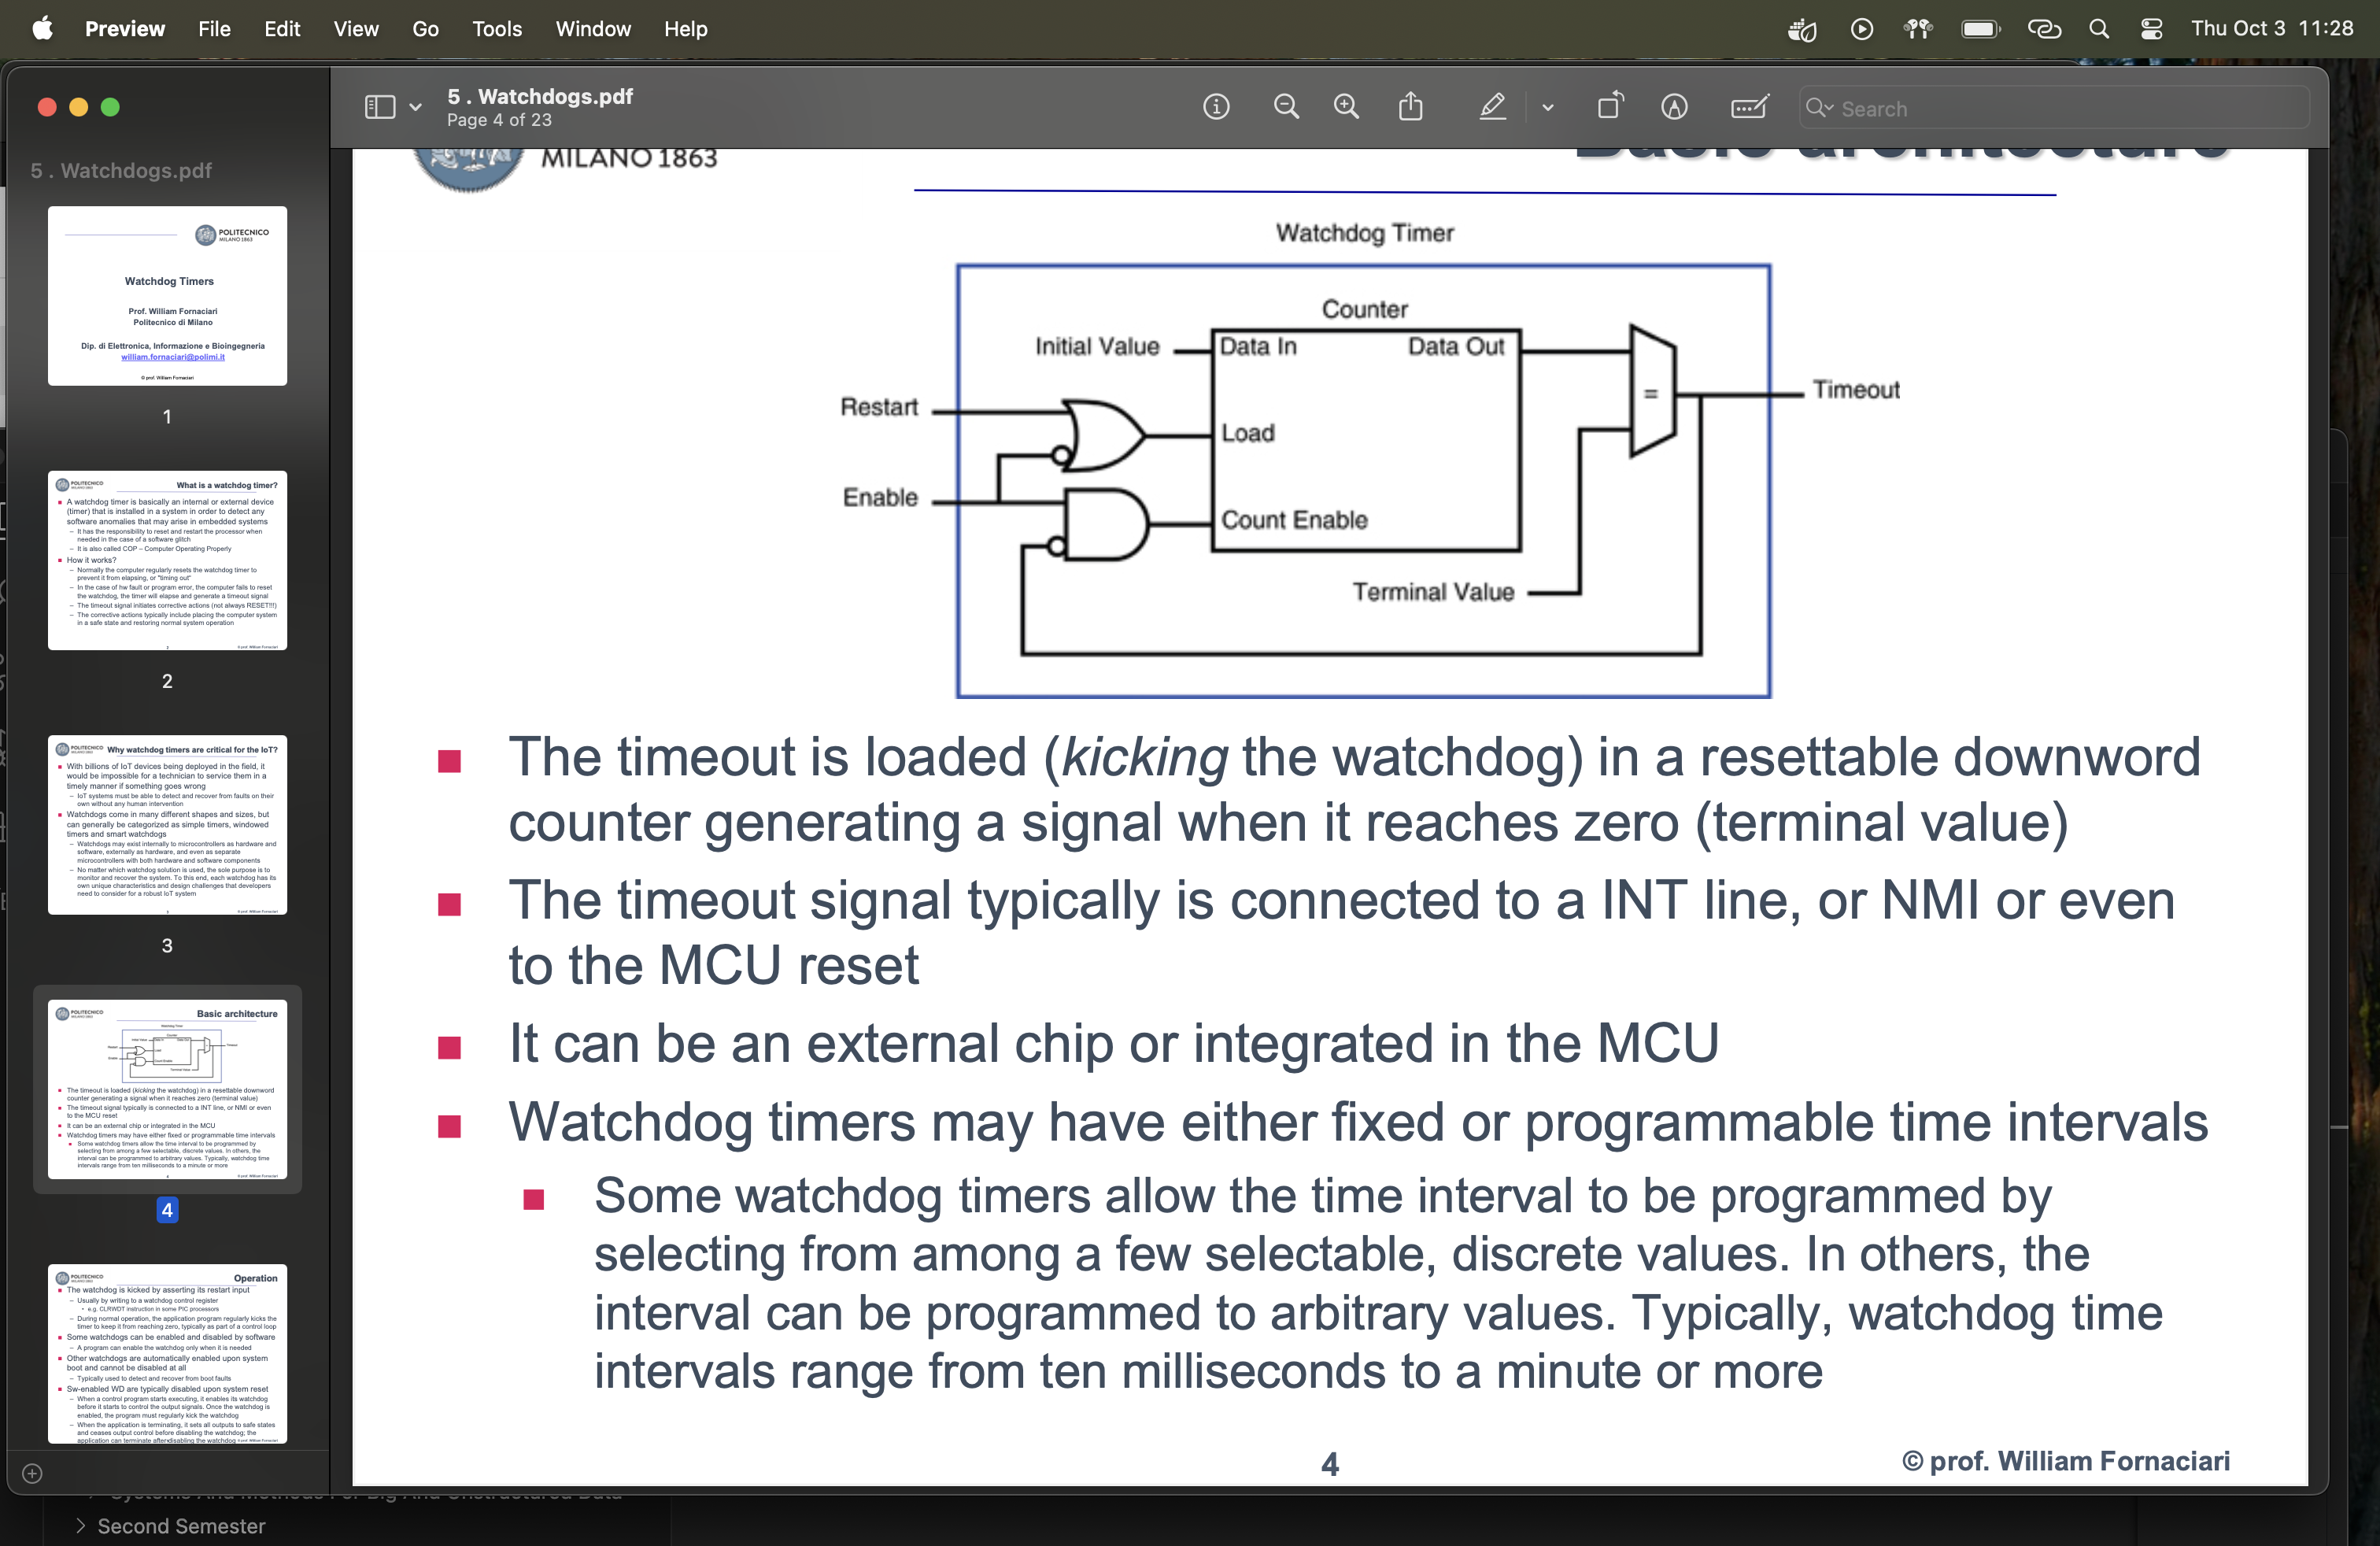
\includegraphics[width=0.75\linewidth]{images/wdog.png}
    \caption{Watchdogs architecture}
\end{figure}
The watchdog timer operates as a countdown timer, which is periodically reset by the system (a process often referred to as "kicking" the watchdog). 
When the countdown reaches zero (the terminal value), a timeout signal is generated. 
This signal may be connected to various system components, such as an interrupt line (INT), a non-maskable interrupt (NMI), or the microcontroller's reset input.

Watchdog timers can be implemented as either external chips or integrated within the microcontroller itself. 
They may offer fixed or programmable timeout intervals. 
In some cases, the interval is selectable from discrete values, while in others, it can be programmed to arbitrary values. 
Typically, the timeout intervals range from milliseconds to minutes, depending on the application.

The watchdog is reset by writing to a dedicated watchdog control register. 
During normal operation, the application continually kicks the watchdog as part of its control loop to prevent the timer from expiring.

\paragraph*{Activation}
Some watchdog timers can be enabled or disabled by software. 
A system may enable the watchdog only when it is needed, while in other cases, watchdogs are automatically activated upon system boot and cannot be disabled. 
Such watchdogs are particularly useful for detecting faults that occur during the boot process.
When a system resets, watchdog timers that are software-enabled are typically disabled until the control program explicitly enables them.
After enabling the watchdog, the system must regularly kick it to prevent a timeout. 
When the application is terminating, it should disable the watchdog after safely shutting down all outputs and stopping control operations.

\paragraph*{Correction}
When a fault is detected, the watchdog initiates one of two main corrective actions:
\begin{enumerate}
    \item \textit{safe state transition}: the system immediately sets all control outputs to safe levels, particularly for devices like motors or heaters, to ensure they do not pose a danger to people or equipment. 
        This is a high-priority action that must happen as soon as the fault is detected.
    \item \textit{system recovery}: once the system is in a safe state, normal operation can be restored. 
        This could be as simple as restarting the system, much like a human pressing a reset button, or it could involve a more complex sequence of steps leading to a reboot.
\end{enumerate}
A watchdog timer is invaluable because it can respond to faults more quickly than a human operator, making it particularly useful in scenarios where immediate action is needed. 
Additionally, watchdog timers can be employed to limit CPU usage for untrusted code running in a sandbox environment, thereby preventing certain types of denial-of-service (DoS) attacks.

\subsection{Single-stage watchdog}
A single-stage watchdog timer is a straightforward design where an immediate system restart is triggered upon timeout. 
In this architecture, the timeout signal is typically connected directly to the computer's system reset input, either via a direct connection or through a conditioning circuit.
When the watchdog times out, it forces a computer restart.

The system relies on this reset to bring the control outputs to their safe states.
Some computers may power down if a continuous timeout signal is sent to the reset input. 
In such cases, a pulse may be required to trigger a system restart, which can be achieved using a pulse generator.
Both the microcontroller and the watchdog timer may share the same clock signal for synchronized operation.
\begin{figure}[H]
    \centering
    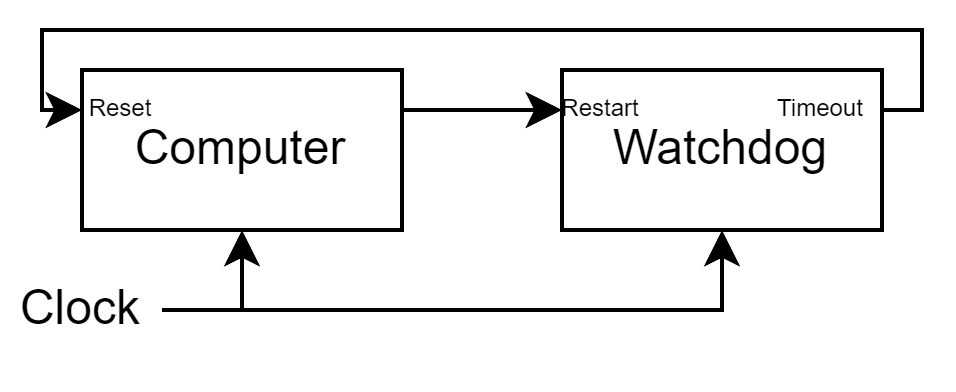
\includegraphics[width=0.5\linewidth]{images/swdog.png}
    \caption{Single stage watchdog}
\end{figure}

\subsection{Multi-stage watchdog}
A multi-stage watchdog consists of two or more timers arranged in a cascade. 
Only the first stage is reset by the processor, and upon its timeout, subsequent stages are initiated, each triggering corrective actions before starting the next stage.

Upon the timeout of the final stage, no further stages are initiated, and typically a full system restart is triggered.
While single-stage watchdog timers are used primarily to restart the computer, multi-stage watchdogs enable a series of corrective actions that happen in stages before restarting the system.
\begin{figure}[H]
    \centering
    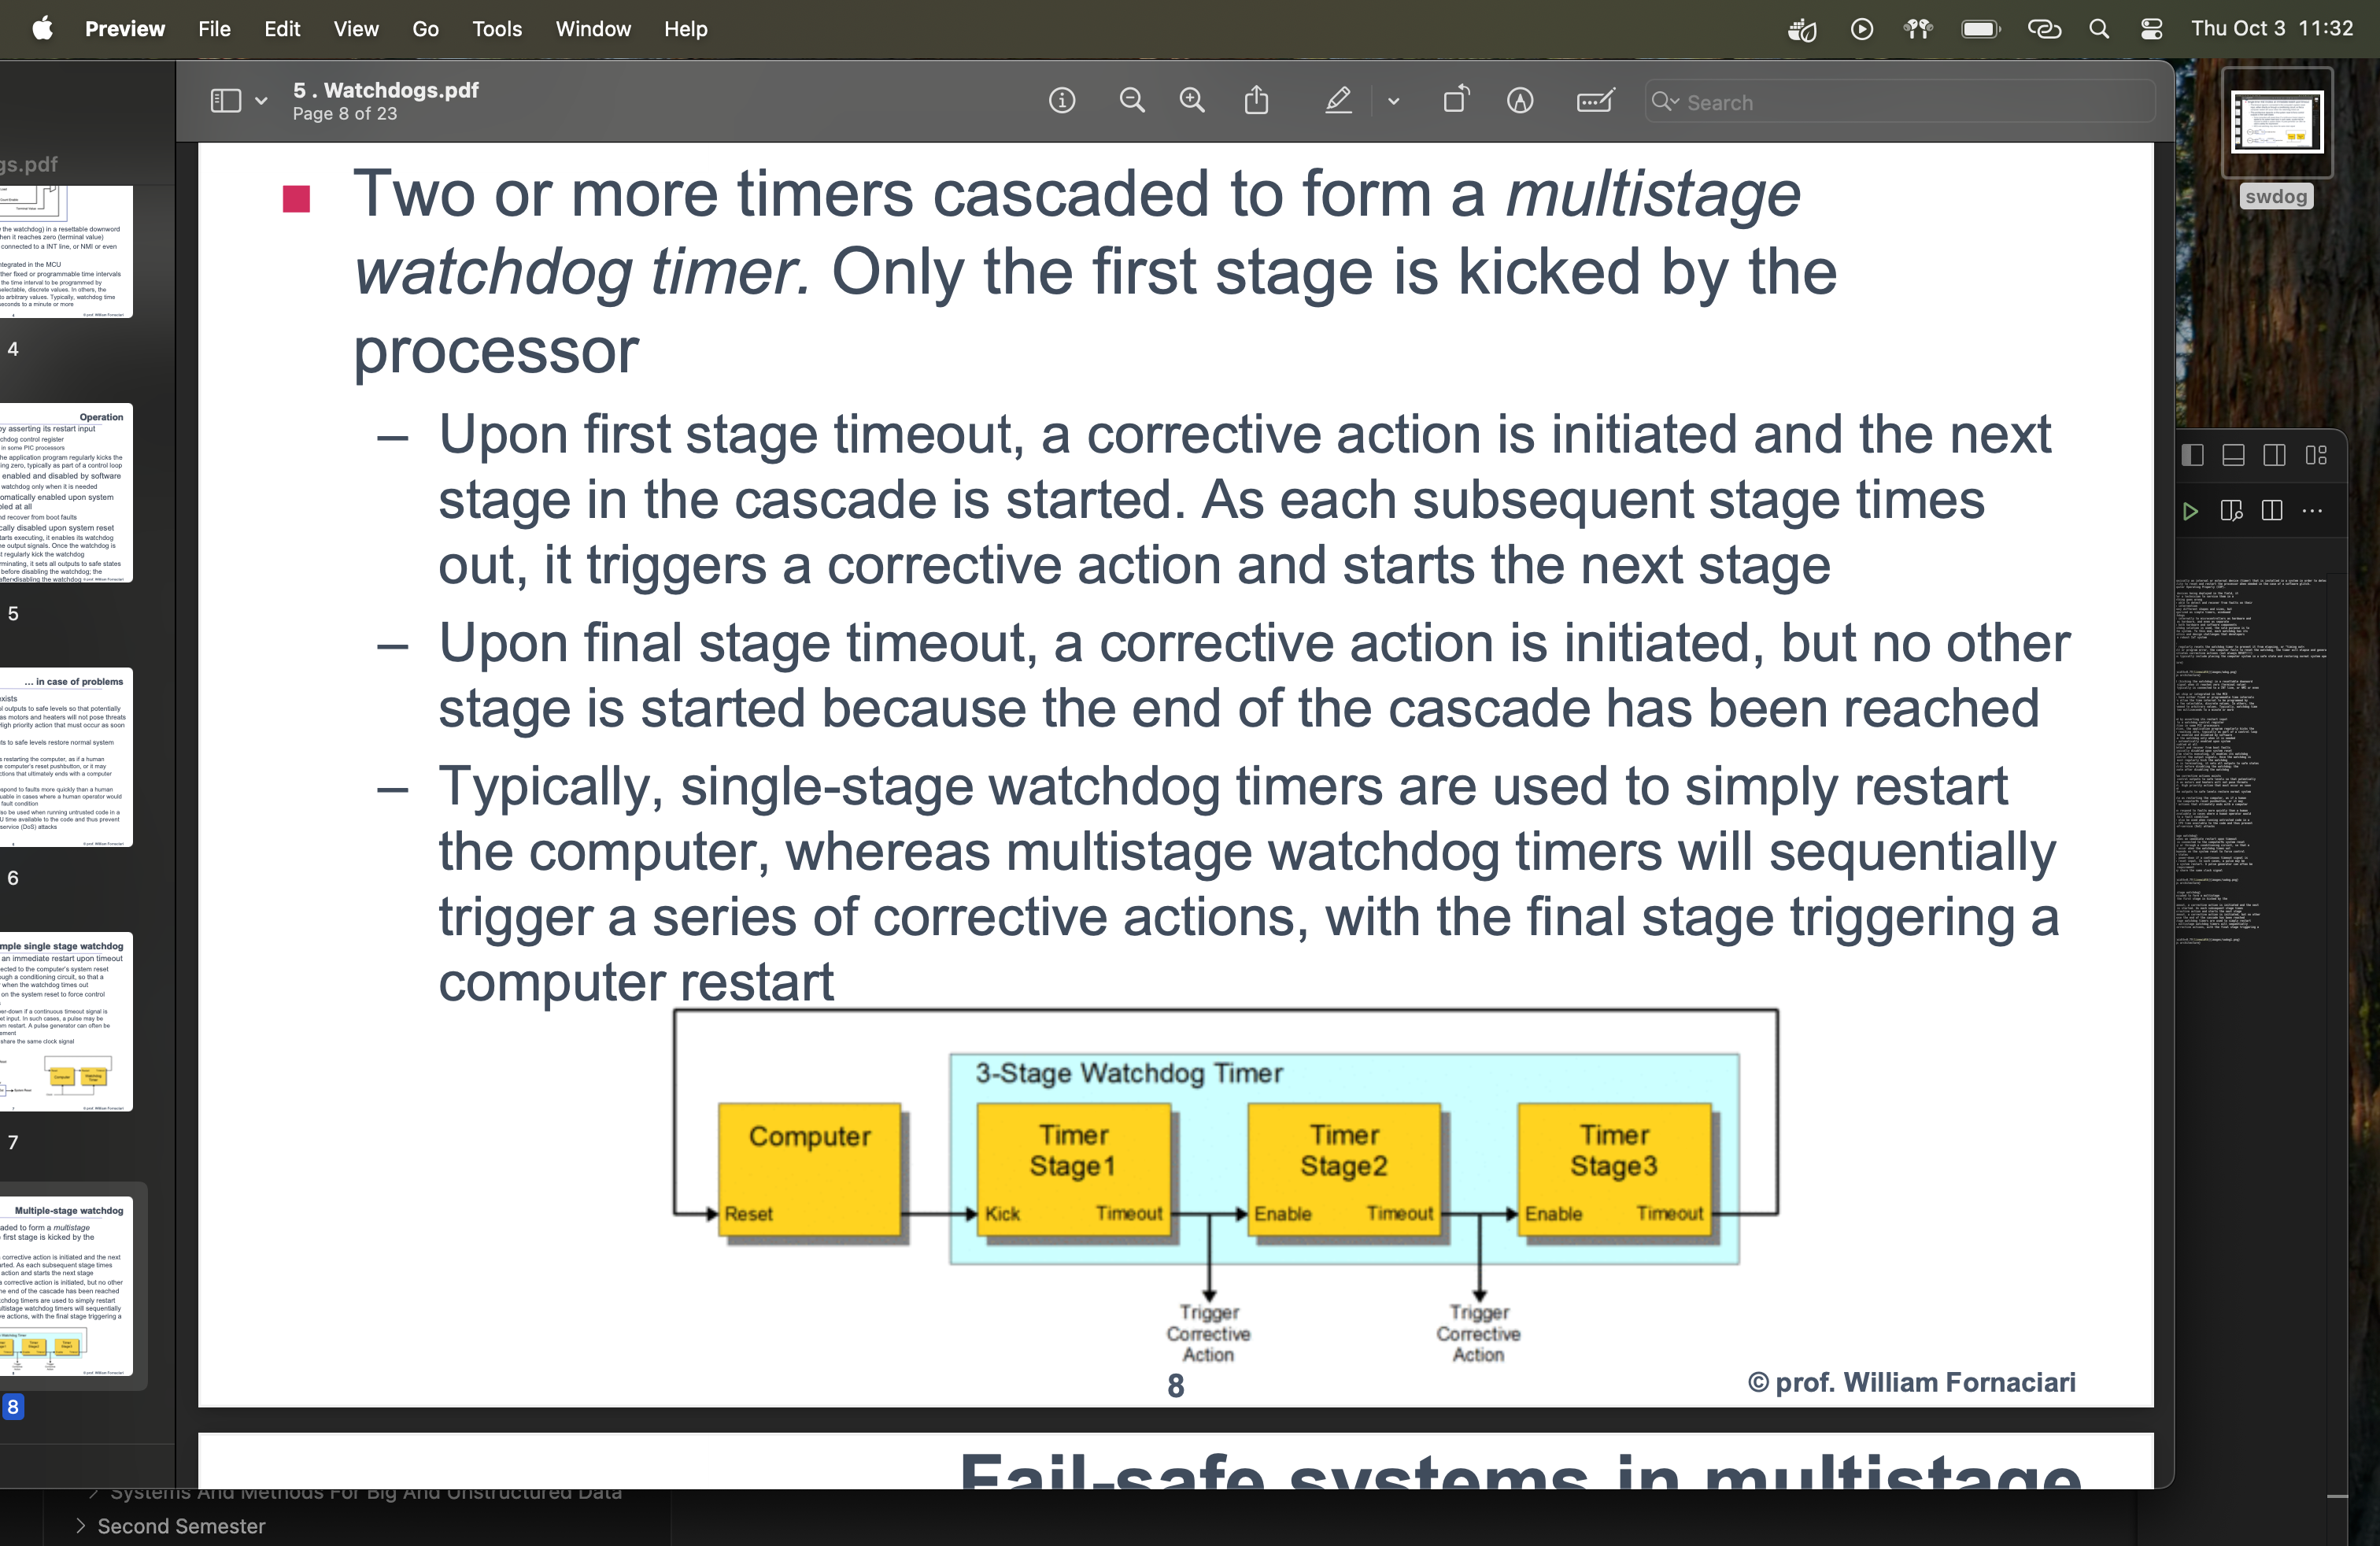
\includegraphics[width=0.75\linewidth]{images/swdog1.png}
    \caption{Multiple stage watchdog}
\end{figure}
Unlike single-stage designs, a multi-stage watchdog does not immediately restart the microcontroller. 
Instead, it schedules a restart, allowing time for corrective actions, such as switching outputs to safe states, to take place.
This staggered approach helps prevent potential hazards and gives the system time to log or recover from errors.

A common technique in multi-stage designs is using a dedicated control reset signal, which resets the control circuitry without resetting the computer itself. 
This avoids the complications of losing critical state information needed for fault recovery.

\paragraph*{mode}
The system operates in two primary modes:
\begin{itemize}
    \item \textit{Run mode}: normal operation where outputs are controlled and managed by the program.
    \item \textit{Safe mode}: a mode in which outputs are placed in pre-defined safe states, typically activated during fault conditions.
\end{itemize}
While the program can modify run mode states at any time, safe mode states can only be changed through a special write-protection mechanism. 
During normal operation, run mode states are sent to the outputs. 
However, when the watchdog times out, the data selector switches to safe mode states to ensure the system is safe.
Since the control circuitry remains operational, it retains vital state information, such as encoder counts and hardware configuration, which may be needed for fault recovery.
\begin{figure}[H]
    \centering
    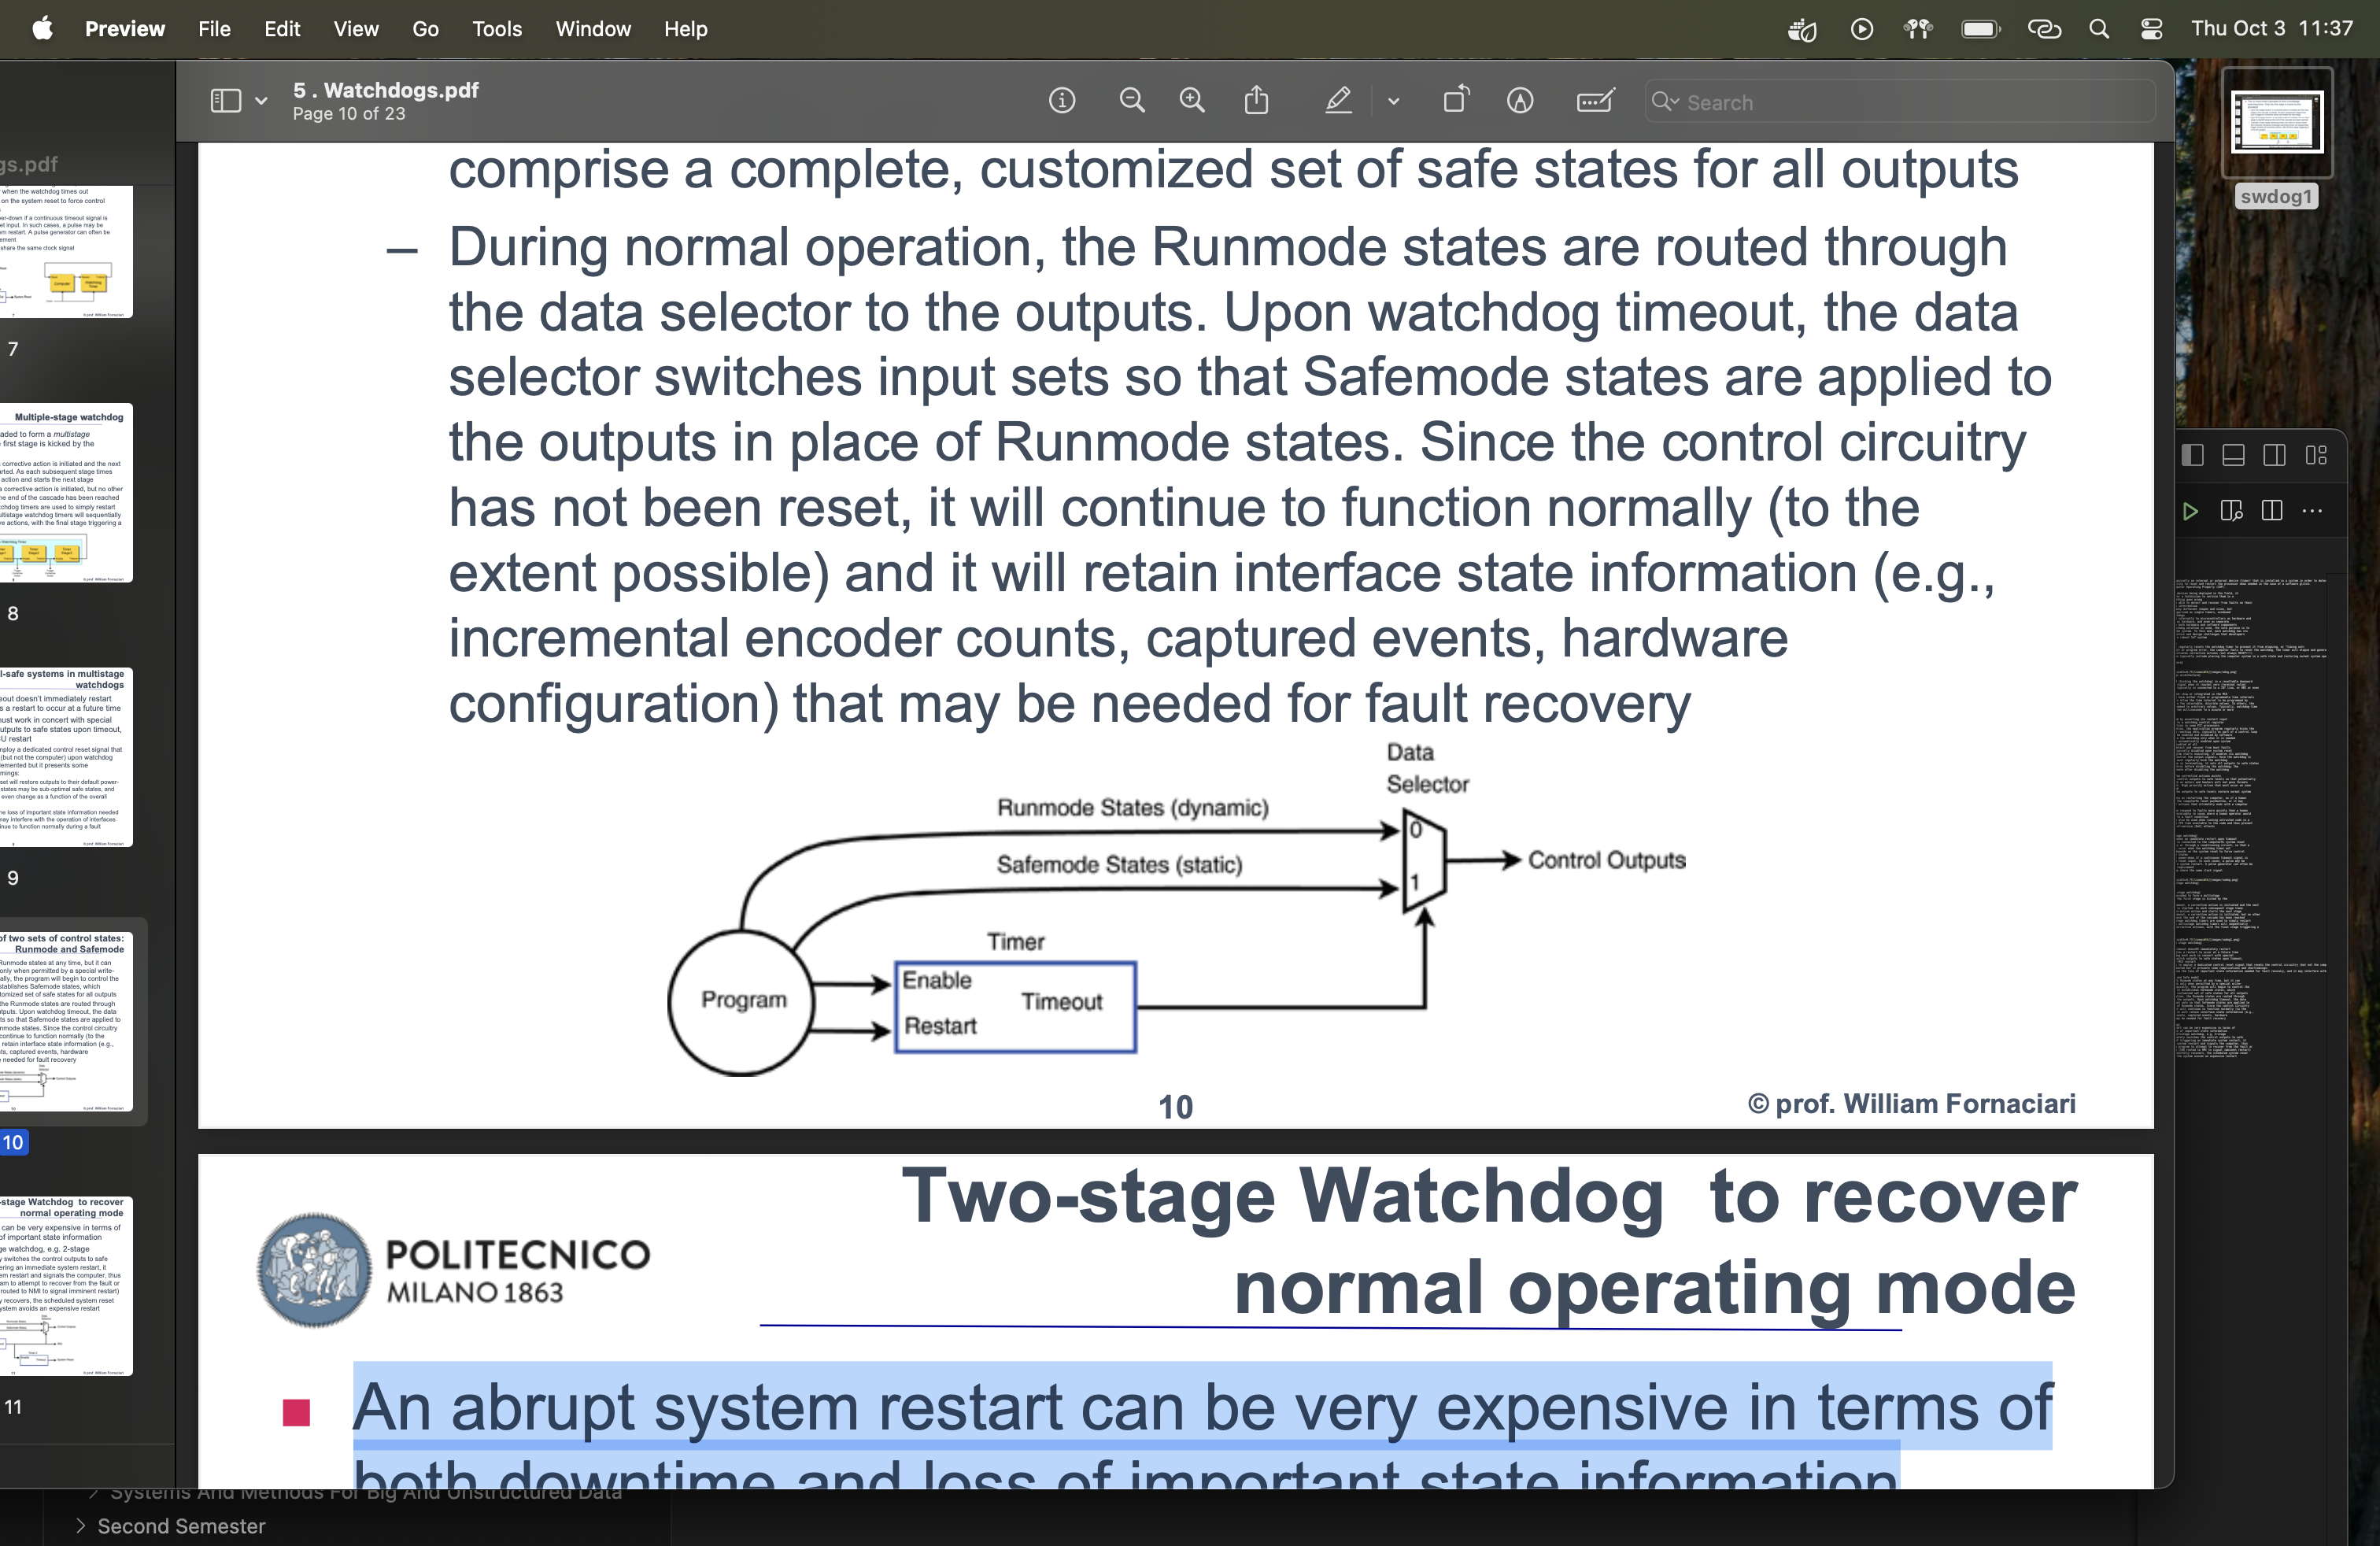
\includegraphics[width=0.75\linewidth]{images/wdog1.png}
    \caption{Watchdog mode}
\end{figure}

\paragraph*{Three-stage watchdog}
In a three-stage watchdog system, Timer1 is responsible for normal operation and regularly gets kicked. 
If Timer1 times out:
\begin{itemize}
    \item It switches the system outputs to safe states, starts Timer2, and requests an interrupt service (IRQ).
    \item If the system responds to the IRQ, the program can attempt to recover from the fault, potentially canceling further corrective actions.
    \item If the system does not respond to the IRQ, Timer2 times out, starts Timer3, and asserts a Non-Maskable interrupt (NMI) to signal an imminent restart. 
        At this stage, important fault information, such as a crash dump, can be logged before the restart.
\end{itemize}
\begin{figure}[H]
    \centering
    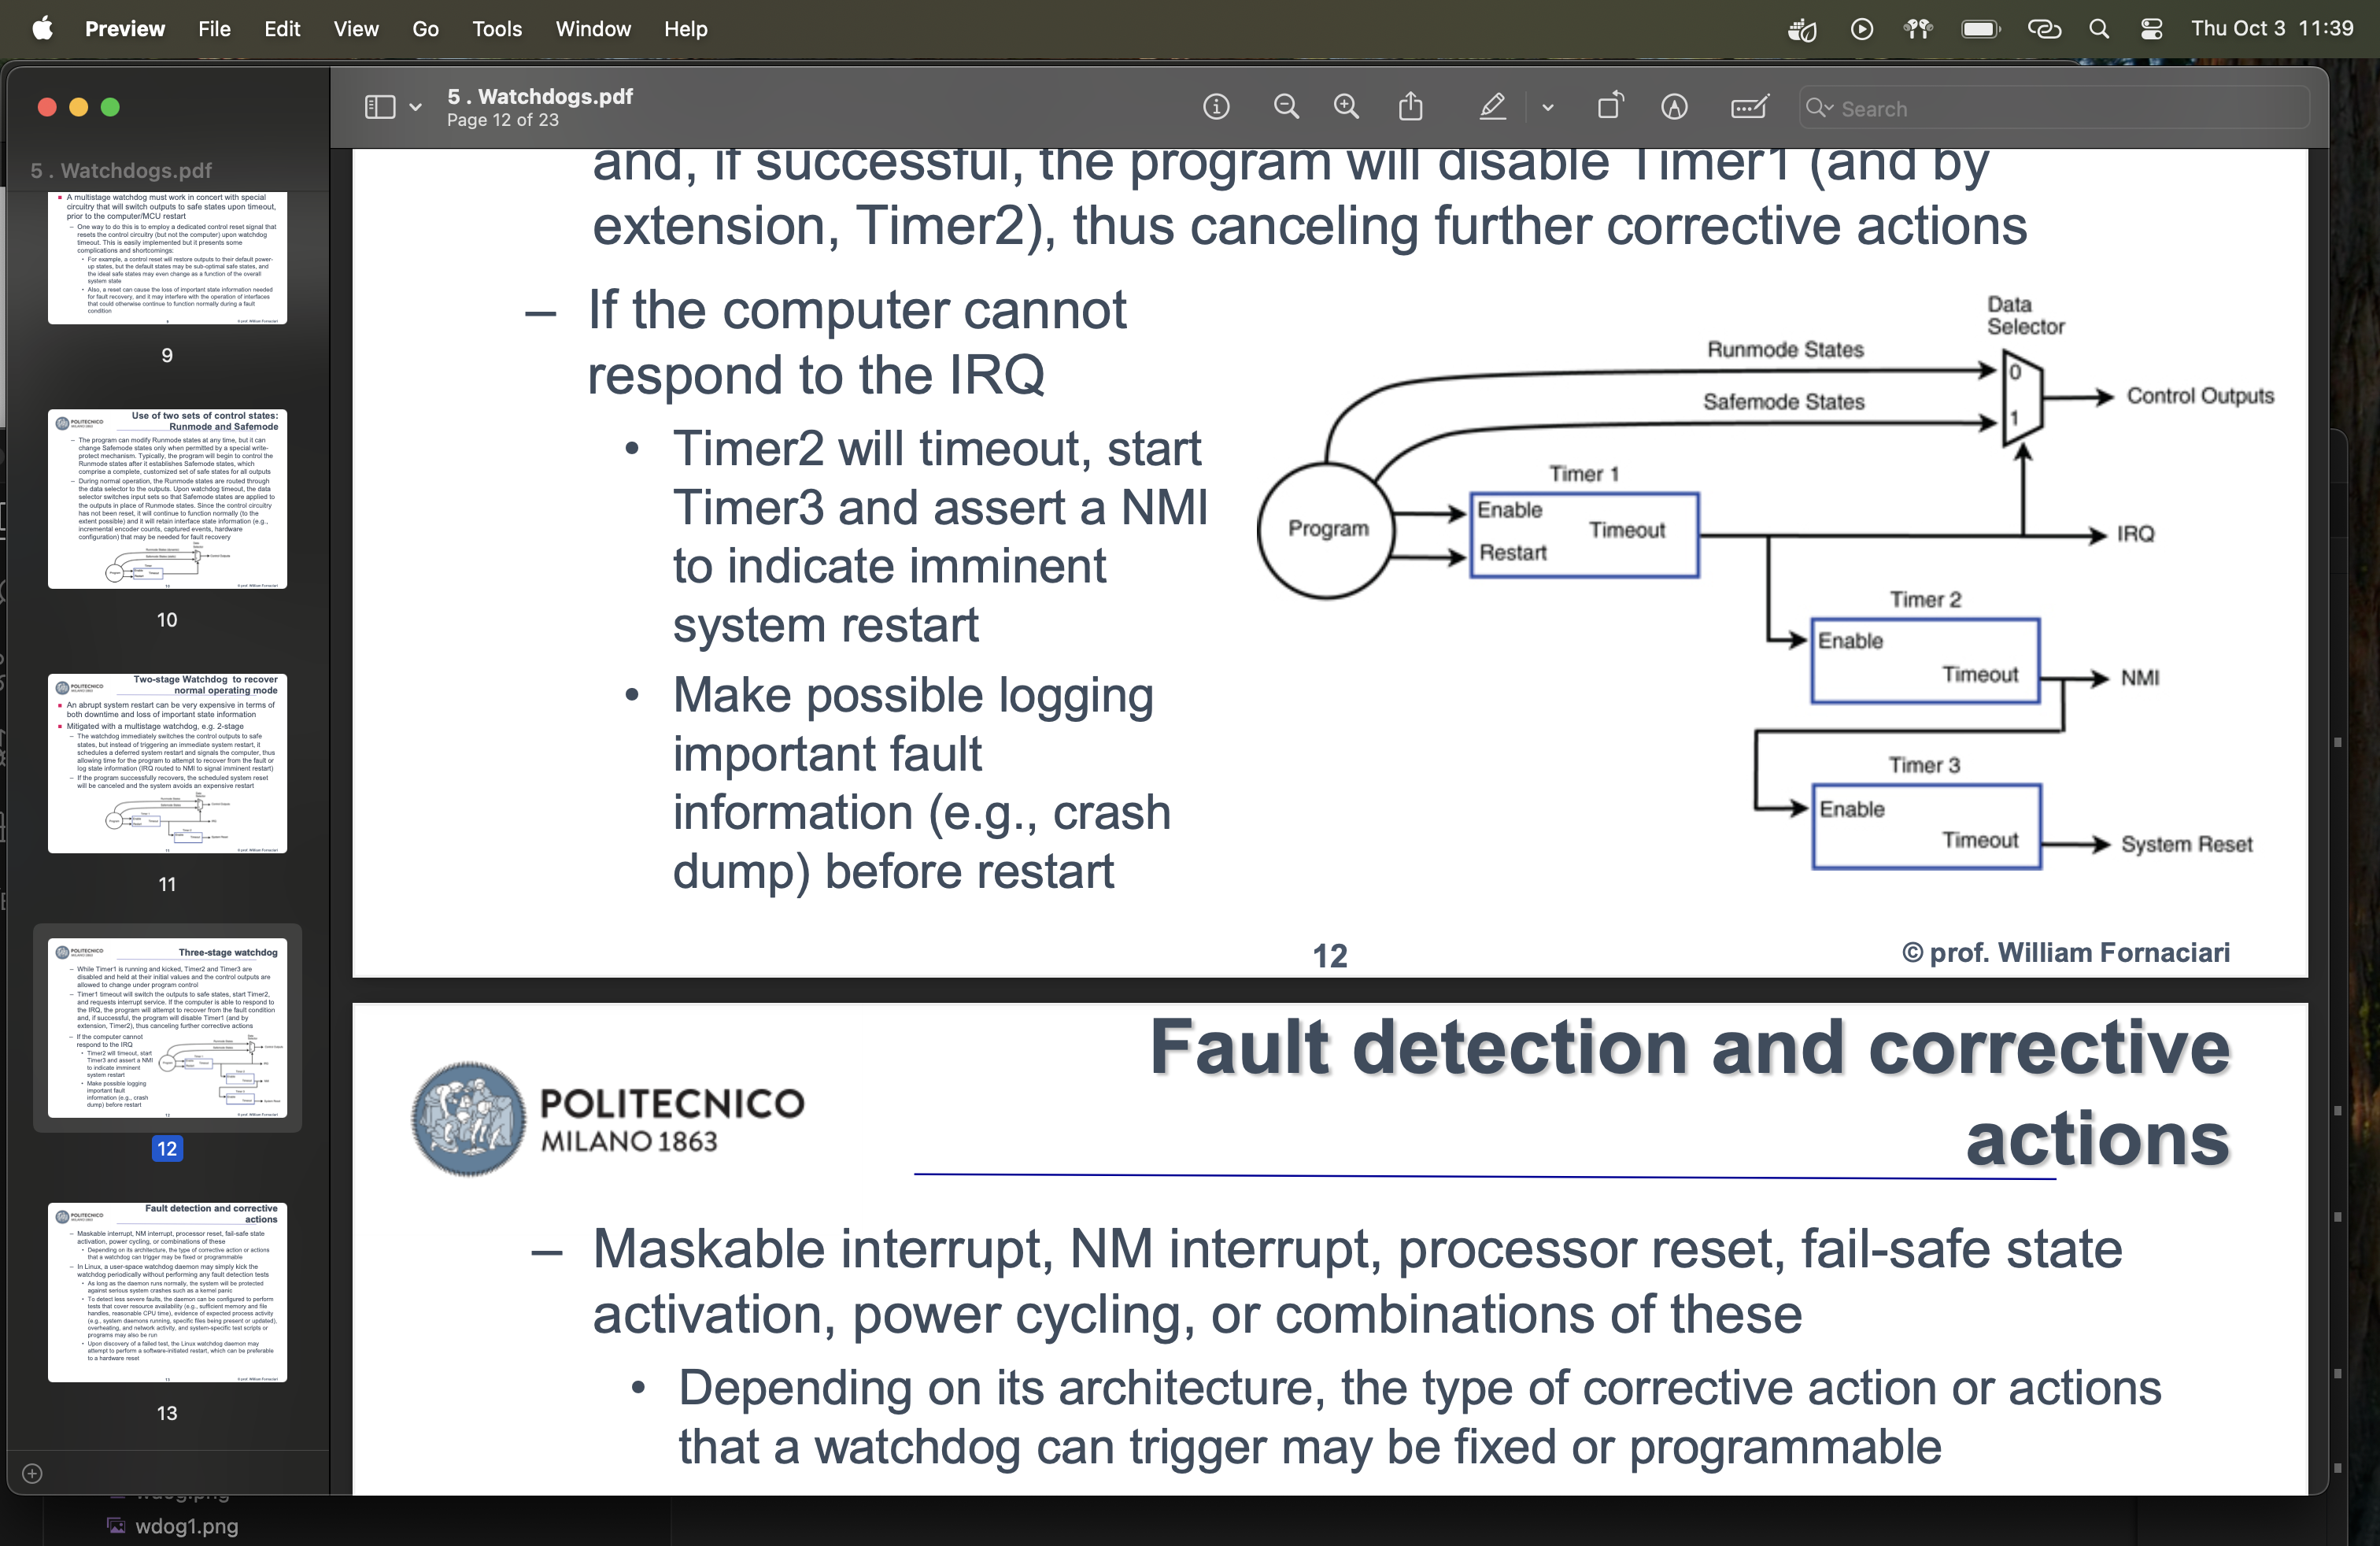
\includegraphics[width=0.75\linewidth]{images/wdog3.png}
    \caption{Three-stage watchdog}
\end{figure}

\paragraph*{Fault detection}
Watchdog timers can trigger various corrective actions, including maskable interrupts, non-maskable interrupts, processor resets, fail-safe state activations, power cycling, or combinations of these, depending on the system architecture.
In Linux systems, a user-space watchdog daemon may periodically reset the watchdog timer without performing extensive fault detection. 
However, to catch less severe issues, the daemon can be configured to monitor resource availability and expected process activity, running specific tests or scripts to detect system abnormalities.
Upon detecting a fault, the daemon may initiate a software reset, which can be preferable to a hardware reset as it allows for a less disruptive recovery process.

\paragraph*{Fault recovery}
Abrupt system restarts due to watchdog timeouts can be costly, both in terms of downtime and the potential loss of important state information. A multi-stage watchdog mitigates this by providing a more controlled recovery process:
\begin{itemize}
    \item The watchdog switches control outputs to safe states immediately.
    \item Rather than an immediate restart, the watchdog schedules a deferred restart and signals the computer, allowing the program time to attempt recovery or log critical state information.
    \item If recovery is successful, the scheduled restart can be canceled, avoiding unnecessary downtime.
\end{itemize}
\begin{figure}[H]
    \centering
    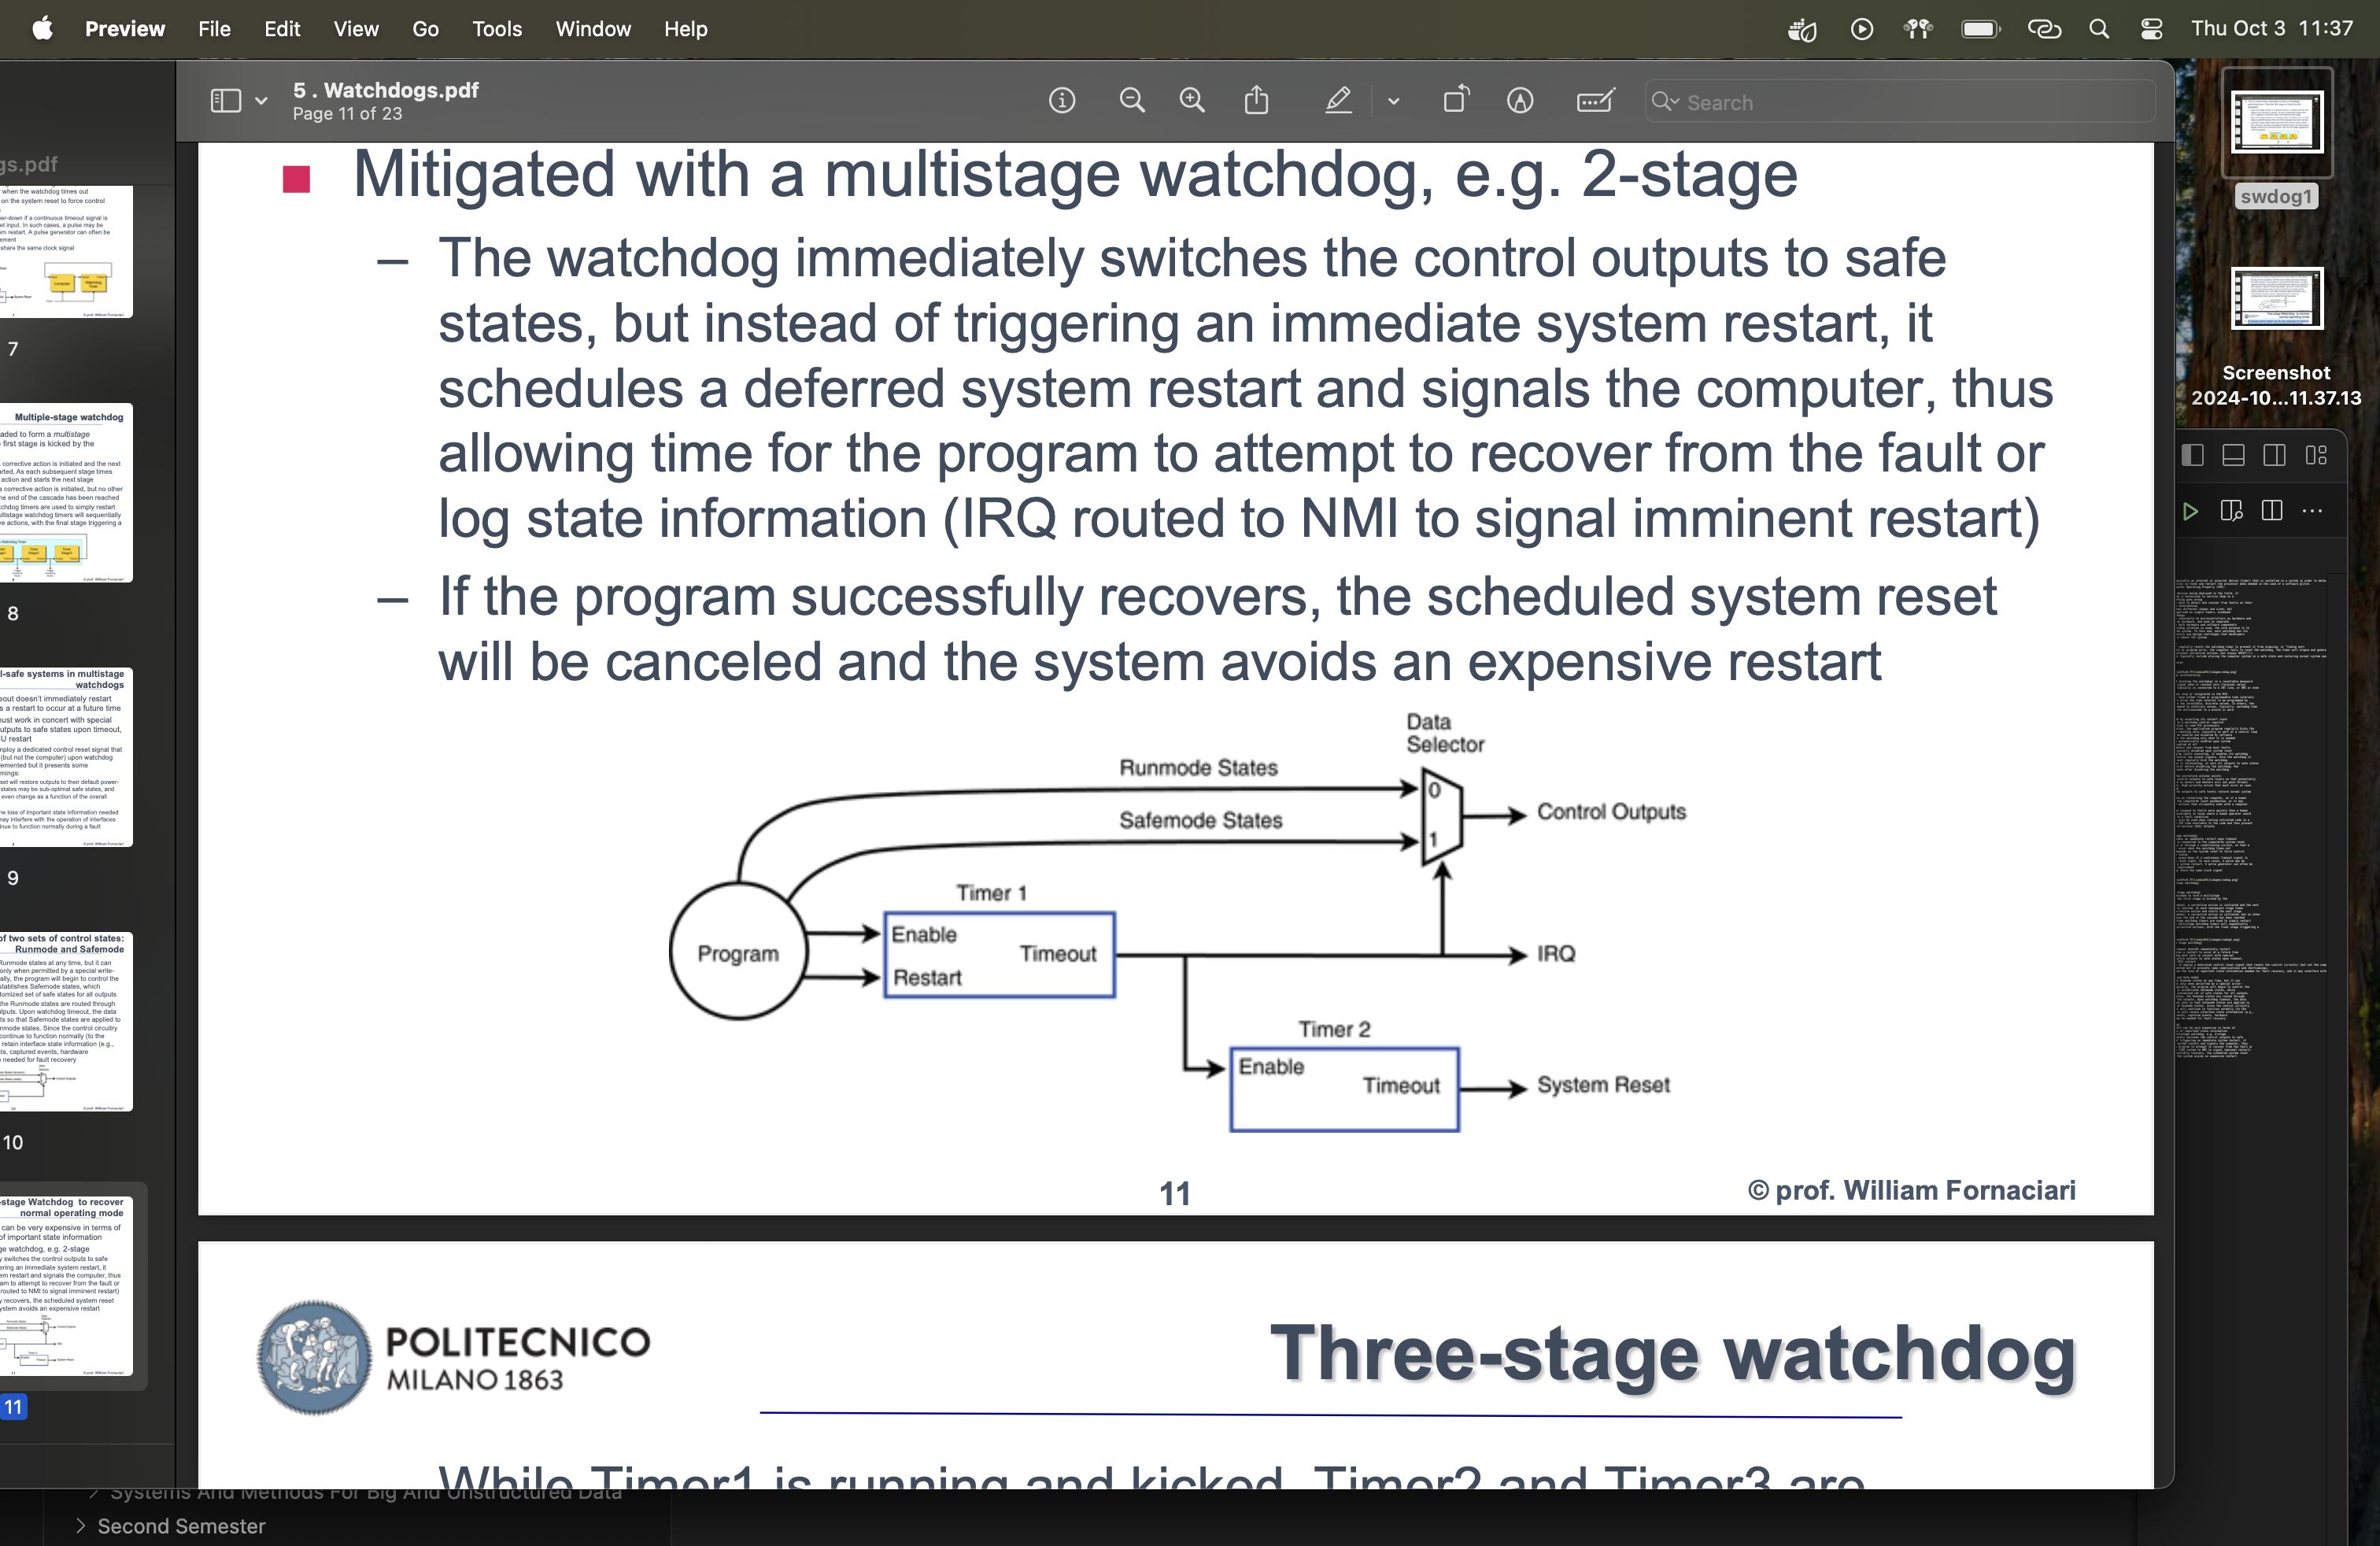
\includegraphics[width=0.75\linewidth]{images/wdog2.png}
    \caption{Watchdog recovery}
\end{figure}

\subsection{AVR watchdog}
AVR devices are equipped with an Enhanced Watchdog Timer (WDT), which operates independently of the main system clock using a dedicated 128kHz on-chip oscillator. 
The WDT acts as a counter that increments with each clock cycle from the oscillator, forcing an interrupt or a system reset once the counter reaches a pre-configured timeout value. 
This timeout can be adjusted within a range of 16 milliseconds to 8 seconds.

In normal operation, the application code must issue a Watchdog Timer reset (WDR) instruction to reset the counter before it reaches the timeout value.
 If this reset does not occur, the system will either generate an interrupt or trigger a system reset, depending on the selected watchdog mode.
There are three primary modes in which the AVR WDT can operate:
\begin{itemize}
    \item In interrupt mode, when the watchdog timer expires, it generates an interrupt that can be used to perform various tasks, such as waking the device from sleep or serving as a general system timer. 
        It is enabled by setting the interrupt mode bit (WDIE) in the Watchdog Timer Control Register (WDTCSR).
    \item In system reset mode, when the timer expires, it forces a system reset. 
        This mode is typically used to prevent the system from hanging due to runaway code.
        It ensures that if the program goes awry, the system is reset and restarted, maintaining overall stability. 
        This mode is enabled by setting the system reset mode bit (WDE) in the WDTCSR.
    \item In the interrupt and system reset mode, both an interrupt and a system reset are triggered in sequence. 
        When the watchdog timer expires, an interrupt is generated first, allowing the system to save critical parameters or execute a graceful shutdown. 
        Afterward, a system reset follows to restart the system safely. 
        This dual-mode is enabled when both the interrupt Enable (WDTIE) and system reset Enable (WDE) bits are set.
\end{itemize}

\subsection{Smart watchdogs}
A smart watchdog takes fault detection a step further by functioning as a supervisory microcontroller that monitors not only heartbeat signals but also system communications.

In some cases, the microcontroller might stop responding to network commands, while still resetting the watchdog timer as usual.
A smart watchdog addresses this by monitoring communication lines, such as UART, and can trigger a reset if communication fails. 

Smart watchdogs are particularly useful in complex systems where communication issues might arise without an outright system crash.
 They ensure that the system stays responsive, even when traditional watchdogs fail to detect such issues.

\subsection{External watchdogs}
Internal watchdog timers, while effective, have limitations that may make them unsuitable for all systems. 
An external watchdog offers several advantages that contribute to system robustness.
For instance, it can initiate a hard system reset that power-cycles the entire microcontroller, including its peripherals, ensuring a full system reset. 
Furthermore, since the external watchdog operates independently, it adds an extra layer of fault detection that is not reliant on the microcontroller's oscillator or logic. 
This kind of watchdog provides an autonomous process to monitor the system's health, significantly increasing system reliability.

However, using an external watchdog does come with trade-offs. 
The additional hardware required increases both the complexity of the system and the overall cost, as an external integrated circuit must be incorporated.

\subsection{Best practice for watchdog usage}
To maximize the effectiveness of watchdog timers, several best practices should be followed. Disabling the watchdog for any reason should be avoided, as it opens the system to vulnerabilities. 
Additionally, clearing the watchdog timer in periodic interrupts without first performing functionality checks is a common mistake; this can lead to runaway software overriding the watchdog's safety mechanism.

It's important to use an independent watchdog timer with a separate clock, allowing it to detect when the system clock has halted. Implementing a windowed watchdog is also recommended. 
A windowed watchdog enforces a minimum time delay before the watchdog can be reset. 
This ensures that if runaway software tries to clear the watchdog too quickly, the system will still be reset.

While internal watchdog timers offer a good starting point for creating a robust embedded system, they are often not enough on their own. 
To achieve greater reliability, external watchdog timers should be considered, particularly in mission-critical applications where failure is not an option.